%% AMS-formatted version of the manuscript
%% Uses the ametsocV6.1 class from AMS LaTeX Package V6.1
%% Version 6.1, 1 September 2021
%
%%%%%%%%%%%%%%%%%%%%%%%%%%%%%%%%%%%%%%%%%%%%%%%%%%%%%%%%%%%%%%%%%%%%%
% PREAMBLE
%%%%%%%%%%%%%%%%%%%%%%%%%%%%%%%%%%%%%%%%%%%%%%%%%%%%%%%%%%%%%%%%%%%%%

% 1.5-SPACED VERSION FOR SUBMISSION TO THE AMS (draft enables line numbering)
\documentclass{ametsocV6.1}

% TWO-COLUMN JOURNAL PAGE LAYOUT---FOR AUTHOR USE ONLY
% \documentclass[twocol]{ametsocV6.1}

%%%%%%%%%%%%%%%%%%%%%%%%%%%%%%%%

% --- Additional packages (beyond what ametsocV6.1 provides) ---
\usepackage{graphicx}
\usepackage{multirow}
\usepackage{subcaption}
\usepackage[section]{placeins}   % keep floats in their section
\usepackage{lineno}              % line numbering for peer review

\graphicspath{{figures/}}

%%%%%%%%%%%%%%%%%%%%%%%%%%%%%%%%

%%% Title

\title{Historical Forecasts vs.\ Reanalysis as Training Data for Machine Learning
Temperature Post-Processing: A Multi-Station, Multi-Architecture Comparison}

%%% Authors and Affiliations
%% Use \correspondingauthor{} and \thanks{} commands
%% \correspondingauthor{} is NECESSARY.
%% Use \aff{#} to indicate the affiliation letter.

\authors{Syed Ali Asad,\aff{a}\correspondingauthor{Syed Ali Asad, syed.asad@s.amity.edu}
Dr.\ Shalini Agarwal,\aff{a}
Syed Mohammad Qasim,\aff{b}
Akram Tariq Khan,\aff{c}
 and Karnav Shah\aff{d}
}

\affiliation{\aff{a}{Amity Institute of Engineering Technology, Amity University Lucknow, Lucknow, India}\\
\aff{b}{Department of Computer Science, Boston University, Boston, USA}\\
\aff{c}{$<$Affiliation$>$}\\
\aff{d}{$<$Affiliation$>$}
}

%%%%%%%%%%%%%%%%%%%%%%%%%%%%%%%%%%%%%%%%%%%%%%%%%%%%%%%%%%%%%%%%%%%%%
% ABSTRACT
%
% Abstracts should not exceed 250 words in length!
%

\abstract{Model Output Statistics (MOS) has been the standard approach for post-processing
numerical weather prediction (NWP) output since the 1970s, traditionally trained
on actual past forecasts. Modern machine learning (ML) practitioners, however,
commonly default to ERA5 reanalysis as training data because of its global coverage
and ease of access. This study systematically evaluates whether training data source
matters for ML-based temperature post-processing by comparing historical forecast
data against ERA5
reanalysis across 28~U.S.\ stations spanning six climate types, five ML architectures
(linear regression, multilayer perceptron, XGBoost, LightGBM, CatBoost), and six
training windows (1--8 years). Over 2{,}200 experiments with block-bootstrap
confidence intervals and Wilcoxon signed-rank tests, we find that:
(1)~historical forecasts reduce mean absolute error (MAE) by 6--26\% compared to
reanalysis for every architecture tested ($p < 0.01$ in 9 of 10 cases);
(2)~simple models (linear regression, MLP) match or outperform gradient-boosted
trees ($p < 0.001$);
(3)~three years of recent data suffices for near-optimal performance; and
(4)~the best ML post-processing reduces MAE by 35\% over raw GFS and 52\% over
raw NWP blends. A feature ablation study across 2{,}240~runs confirms that core NWP
predictors and bias-correction features are essential, while lagged observations
and rolling statistics can harm tree-based models. These results provide practical
guidance for operational weather prediction and the growing weather derivatives
market.}

\begin{document}

%% Necessary!
\maketitle

%% Enable line numbering (required for AMS submission)
\linenumbers

%%%%%%%%%%%%%%%%%%%%%%%%%%%%%%%%%%%%%%%%%%%%%%%%%%%%%%%%%%%%%%%%%%%%%
% SIGNIFICANCE STATEMENT
%%%%%%%%%%%%%%%%%%%%%%%%%%%%%%%%%%%%%%%%%%%%%%%%%%%%%%%%%%%%%%%%%%%%%

\statement
Machine learning post-processing of weather forecasts is increasingly common,
yet the fundamental question of what training data to use has been overlooked.
We demonstrate that training on historical forecasts rather than reanalysis
reduces temperature prediction errors by 6--26\% across all model architectures,
and that simple linear models match or outperform complex gradient-boosted trees.
These findings challenge the widespread use of ERA5 reanalysis and complex ML
architectures, providing actionable guidance for operational forecasters and
weather prediction market participants.

%%%%%%%%%%%%%%%%%%%%%%%%%%%%%%%%%%%%%%%%%%%%%%%%%%%%%%%%%%%%%%%%%%%%%
% MAIN BODY OF PAPER
%%%%%%%%%%%%%%%%%%%%%%%%%%%%%%%%%%%%%%%%%%%%%%%%%%%%%%%%%%%%%%%%%%%%%

\section{Introduction}
\label{sec:intro}

Statistical post-processing of numerical weather prediction (NWP) output---known
as Model Output Statistics (MOS)---has been a cornerstone of operational weather
forecasting since \citet{glahn1972mos} introduced the technique at the U.S.\
National Weather Service. The core insight of MOS is straightforward: by training
statistical models on the relationship between past NWP forecasts and corresponding
observations, systematic biases and deficiencies in the NWP model can be corrected,
yielding forecasts that consistently outperform the raw NWP guidance
\citep{carter1989mos, wilks2011statistical}.

In recent years, machine learning (ML) methods have been increasingly applied to
weather post-processing, with gradient-boosted trees
\citep{taillardat2016calibrated}, neural networks \citep{rasp2018neural}, and other
nonlinear models demonstrating skill improvements over classical linear MOS
\citep{vannitsem2021statistical, schulz2022machine}. These advances have been
accompanied by growing interest in weather prediction markets, where platforms
such as Kalshi and Polymarket offer daily contracts on maximum and minimum
temperatures at major U.S.\ airports, with annual trading volumes exceeding
\$200~million \citep{snowberg2013prediction}.

Despite the maturation of ML-based post-processing, a critical but under-examined
choice faces every practitioner: \emph{what data should the model be trained on?}
Classical MOS was always trained on actual past forecasts---the very NWP output the
model seeks to correct. However, the modern ML community has largely converged on
ERA5 reanalysis \citep{hersbach2020era5} as the default training data source, drawn
by its global coverage, temporal completeness, and free availability. The implicit
assumption is that reanalysis adequately captures the statistical relationship
between atmospheric state and surface weather.

This assumption is questionable. Reanalysis represents the atmosphere's best
estimate of what \emph{actually happened}, not what the forecast model
\emph{predicted would happen}. Forecast-specific biases---systematic errors tied to
the NWP model's physics, resolution, and parameterizations---are absent from
reanalysis. If these biases are learnable and correctable, training on historical
forecasts should outperform training on reanalysis, regardless of model architecture.

No published study has systematically quantified this effect across stations,
climates, model architectures, and training data volumes using freely available
APIs. This paper fills that gap with the following contributions:

\begin{enumerate}
  \item A controlled comparison of historical forecasts vs.\ ERA5 reanalysis as
    training data across 28~stations, five ML architectures, and six climate types,
    showing a statistically significant 6--26\% MAE reduction with historical
    forecasts for every architecture tested ($p < 0.01$).
  \item An architecture comparison demonstrating that simple models (linear
    regression, MLP) match or outperform gradient-boosted trees for temperature
    post-processing.
  \item Training window sensitivity analysis showing that 3--5~years of recent
    historical forecast data is optimal.
  \item A feature ablation study (2{,}240~runs) identifying which feature groups
    contribute to---or detract from---post-processing skill.
  \item Quantification of MOS skill relative to raw NWP: the best ML model
    reduces MAE by 35\% over raw GFS output.
\end{enumerate}

All experiments use the same fixed test period (July 2025--February 2026), the same
48-feature engineering pipeline, and the same evaluation framework with
block-bootstrap confidence intervals and paired nonparametric significance tests.

% ======================================================================
\section{Related Work}
\label{sec:related}

\subsection{Classical MOS and Statistical Post-Processing}

MOS was introduced by \citet{glahn1972mos} and has been operational at the U.S.\
National Weather Service since the early 1970s. The foundational principle is that
regression models trained on past forecast--observation pairs can systematically
correct NWP biases \citep{carter1989mos}. \citet{wilks2011statistical} provides a
comprehensive treatment of statistical post-processing methods, including MOS,
perfect-prog, and analog approaches.

\citet{vannitsem2021statistical} review the current state of statistical
post-processing in a ``big data world,'' noting that while classical methods remain
operationally robust, modern ML techniques offer opportunities for improvement,
particularly in capturing nonlinear forecast--observation relationships. A key
observation from this review is that the choice of training data---actual forecasts
vs.\ reanalysis vs.\ analysis fields---is often treated as incidental rather than
as an experimental variable.

\subsection{Machine Learning for Weather Post-Processing}

The application of ML to weather post-processing has accelerated rapidly.
\citet{taillardat2016calibrated} demonstrated that quantile regression forests
outperform classical ensemble MOS (EMOS) for calibrating ensemble precipitation
forecasts. \citet{rasp2018neural} showed that neural networks can learn
distributional forecasts from ensemble output, matching or exceeding EMOS skill
for temperature and precipitation.

\citet{mcgovern2017using} provided an early comprehensive overview of ML
applications in operational meteorology, emphasizing the need for interpretable
models and proper evaluation. \citet{schulz2022machine} systematically compared
ML methods for wind gust post-processing, finding that gradient-boosted trees
(particularly XGBoost and LightGBM) and neural networks provide comparable
skill improvements over EMOS.

More recently, \citet{haupt2021first} outlined a roadmap for implementing AI-based
post-processing in operational settings, highlighting challenges including data
quality, computational cost, and the gap between research demonstrations and
operational deployment.

\subsection{Training Data Considerations}

The choice of training data for ML-based post-processing has received surprisingly
little systematic attention. Most modern studies use one of three approaches:
(1)~ERA5 reanalysis \citep{hersbach2020era5} as both predictor and predictand;
(2)~operational analysis fields; or (3)~station observations as predictands with
forecast fields as predictors. The use of \emph{historical forecasts}---actual past
NWP output from operational models like GFS \citep{ncep2021gfs}---as training
predictors has been limited by data availability.

The recent emergence of historical forecast APIs, particularly the Open-Meteo
Historical Forecast API \citep{zippenfenig2023openmeteo}, has made multi-year
archives of past GFS and ECMWF forecasts freely accessible. This removes the
primary barrier to training on historical forecasts and motivates a systematic
comparison with the reanalysis-based approach that has become the community default.

\subsection{Probabilistic Forecasting and Calibration}

Quantile regression \citep{koenker1978quantile} provides a natural framework for
probabilistic post-processing, producing prediction intervals without distributional
assumptions. \citet{romano2019conformal} introduced conformalized quantile
regression, which combines quantile regression with conformal prediction
\citep{romano2019conformal} to produce prediction intervals with finite-sample
coverage guarantees. We adopt this approach for calibrating our prediction intervals.

% ======================================================================
\section{Data and Methods}
\label{sec:methods}

\subsection{Stations}
\label{sec:stations}

We study all 28~U.S.\ cities where daily temperature prediction contracts are
actively traded on the Kalshi exchange, providing the research with direct practical
relevance. These stations span six climate types: Continental (6~stations),
Northeast Coastal (5), Southeast Subtropical (6), Gulf/South Central (6), Pacific
Maritime (3), and Arid (2). Station coordinates, climate classifications, and
identifiers are listed in Table~\ref{tab:stations}.

\begin{table}[t]
\caption{Study stations grouped by climate type. All 28~stations correspond to
active Kalshi daily temperature markets.}\label{tab:stations}
\begin{center}
\begin{tabular}{llrr}
\topline
Climate Type & Station (City) & Lat & Lon \\
\midline
\multirow{6}{*}{Continental}
  & KORD (Chicago O'Hare) & 42.0 & $-$87.9 \\
  & KMDW (Chicago Midway) & 41.8 & $-$87.8 \\
  & KMSP (Minneapolis) & 44.9 & $-$93.2 \\
  & KDTW (Detroit) & 42.2 & $-$83.4 \\
  & KDEN (Denver) & 39.9 & $-$104.7 \\
  & KOKC (Oklahoma City) & 35.4 & $-$97.6 \\
\midline
\multirow{5}{*}{NE Coastal}
  & KNYC (New York) & 40.8 & $-$74.0 \\
  & KLGA (LaGuardia) & 40.8 & $-$73.9 \\
  & KBOS (Boston) & 42.4 & $-$71.0 \\
  & KPHL (Philadelphia) & 39.9 & $-$75.2 \\
  & KDCA (Washington D.C.) & 38.9 & $-$77.0 \\
\midline
\multirow{6}{*}{SE Subtropical}
  & KATL (Atlanta) & 33.6 & $-$84.4 \\
  & KCLT (Charlotte) & 35.2 & $-$80.9 \\
  & KBNA (Nashville) & 36.1 & $-$86.7 \\
  & KJAX (Jacksonville) & 30.5 & $-$81.7 \\
  & KTPA (Tampa) & 28.0 & $-$82.5 \\
  & KMIA (Miami) & 25.8 & $-$80.3 \\
\midline
\multirow{6}{*}{Gulf/SC}
  & KHOU (Houston) & 29.6 & $-$95.3 \\
  & KMSY (New Orleans) & 30.0 & $-$90.3 \\
  & KDFW (Dallas DFW) & 32.9 & $-$97.0 \\
  & KDAL (Dallas Love) & 32.8 & $-$96.9 \\
  & KAUS (Austin) & 30.2 & $-$97.7 \\
  & KSAT (San Antonio) & 29.5 & $-$98.5 \\
\midline
\multirow{3}{*}{Pacific}
  & KLAX (Los Angeles) & 33.9 & $-$118.4 \\
  & KSFO (San Francisco) & 37.6 & $-$122.4 \\
  & KSEA (Seattle) & 47.5 & $-$122.3 \\
\midline
\multirow{2}{*}{Arid}
  & KPHX (Phoenix) & 33.4 & $-$112.0 \\
  & KLAS (Las Vegas) & 36.1 & $-$115.2 \\
\botline
\end{tabular}
\end{center}
\end{table}

\subsection{Data Sources}
\label{sec:data_sources}

\paragraph{Historical Forecasts.}
We retrieve past GFS and ECMWF IFS deterministic forecasts via the Open-Meteo
Historical Forecast API \citep{zippenfenig2023openmeteo}. For each station, we
extract daily maximum and minimum temperature forecasts (2-m temperature), as well
as wind speed, wind direction, dew point, solar radiation, and cloud cover. When
both GFS and ECMWF forecasts are available, we compute a simple mean blend as the
primary predictor and retain the individual model outputs as separate features.

\paragraph{Reanalysis.}
ERA5 reanalysis data \citep{hersbach2020era5} are retrieved through the Open-Meteo
Archive API. We extract the same variables as for historical forecasts, ensuring
a fair comparison of predictor sets.

\paragraph{Observations.}
Actual daily maximum and minimum temperatures are obtained from the Applied Climate
Information System (ACIS), which provides official NWS Climate Data Online
observations. These are the same values used for Kalshi contract settlement.

\paragraph{Fixed test period.}
All experiments use a common test period of 1~July 2025 through 12~February 2026
(approximately 227~days), ensuring that all comparisons are on identical test data.

\subsection{Feature Engineering}
\label{sec:features}

From the raw forecast and observation data, we engineer 48~features organized into
8 groups:

\begin{enumerate}
  \item \textbf{NWP Primary} (6): GFS and blended forecast temperatures
    (MaxT, MinT, MeanT).
  \item \textbf{ECMWF} (4): ECMWF-specific temperatures and forecast uncertainty
    (GFS--ECMWF spread).
  \item \textbf{Bias Correction} (4): Yesterday's forecast error (actual $-$
    forecast) and 3-day rolling mean error, for both MaxT and MinT.
  \item \textbf{Lagged Observations} (6): Observed MaxT and MinT for the previous
    1--3~days.
  \item \textbf{Rolling Statistics} (12): Rolling means (3-day, 7-day), standard
    deviations, momentum, acceleration, and deviation from 30-day mean.
  \item \textbf{NWP Atmosphere} (5): Forecast wind speed, direction, dew point,
    solar radiation, and cloud cover.
  \item \textbf{Physics-Derived} (7): U/V wind components, Chinook index,
    dew-point depression, solar load, clear-sky index, and cooling potential.
  \item \textbf{Time} (4): Sine/cosine of day-of-year, day of week, weekend
    indicator.
\end{enumerate}

\subsection{Model Architectures}
\label{sec:models}

We compare five architectures spanning linear, tree-based, and neural approaches:

\begin{itemize}
  \item \textbf{Linear}: Scikit-learn \texttt{QuantileRegressor} with $L_1$
    penalty, fitting quantiles $\tau \in \{0.25, 0.50, 0.75\}$.
  \item \textbf{MLP}: A two-hidden-layer neural network (PyTorch) with 128 and
    64~units, ReLU activations, dropout, and pinball loss for each quantile.
  \item \textbf{XGBoost}: Gradient-boosted trees \citep{chen2016xgboost} with
    quantile regression objective.
  \item \textbf{LightGBM}: \citet{ke2017lightgbm} with quantile regression.
  \item \textbf{CatBoost}: \citet{prokhorenkova2018catboost} with quantile
    regression and built-in ordered boosting.
\end{itemize}

All models are trained on the same chronological 60/20/20 split (train/validation/test),
with early stopping (100-round patience) on the validation set for iterative models.
Prediction intervals are calibrated using conformalized quantile regression
\citep{romano2019conformal}, targeting 50\% coverage.

\subsection{Evaluation}
\label{sec:evaluation}

\paragraph{Metrics.}
The primary metric is mean absolute error (MAE) of the median ($\tau = 0.50$)
forecast. We also record RMSE, mean bias, and 50\% prediction interval coverage
for each experiment; supplementary RMSE results are provided in Table~\ref{tab:supp_rmse}.

\paragraph{Confidence intervals.}
For each experiment, we compute block-bootstrap confidence intervals
\citep{kunsch1989jackknife} with block size 10~days and 1{,}000 resamples to
account for temporal autocorrelation in forecast errors.

\paragraph{Significance tests.}
Comparisons across 28~stations are evaluated using the Wilcoxon signed-rank test
\citep{wilcoxon1945individual}, a nonparametric paired test appropriate for the
non-normal distribution of MAE differences. We report one-sided $p$-values
(testing whether the hypothesized better method is significantly better).

\paragraph{Experimental scale.}
The full study comprises 2{,}212~main experiments (28~stations $\times$
5~architectures $\times$ 2~targets $\times$ 2~data sources $\times$ multiple
training windows) plus 2{,}240~ablation runs, with zero failures.

% ======================================================================
\section{Results}
\label{sec:results}

\subsection{Data Source Comparison (RQ1--RQ2)}
\label{sec:results_source}

Table~\ref{tab:data_source} compares historical forecasts and ERA5 reanalysis as
training data across all five architectures with a 3-year training window and
28~stations. Historical forecasts yield significantly lower MAE for every
architecture--target combination ($p < 0.01$ in 9 of 10 cases; $p = 0.057$
for LightGBM MinT). The improvement is largest for the simplest models:
MLP gains 26.3\% on MaxT and 19.5\% on MinT, while Linear gains 25.6\%
and 18.3\%, respectively. Even the weakest effect (LightGBM MinT, 5.7\%)
shows a consistent direction. This demonstrates that the data-source
effect is a fundamental property of the MOS training signal, not an
artefact of one particular model family (Fig.~\ref{fig:data_source}).

\begin{table}[t]
\caption{Data source comparison: mean MAE (\textdegree{}F) $\pm$ SE across
28~stations (3-year training window). $p$-values from Wilcoxon signed-rank
test (HF $<$ ERA5). Improvement = $(1 - \text{HF}/\text{ERA5}) \times 100$.}\label{tab:data_source}
\begin{center}
\begin{tabular}{llcccc}
\topline
Target & Architecture & Hist.\ Forecast & ERA5 Reanalysis & Improv.\ (\%) & $p$ \\
\midline
\multirow{5}{*}{MaxT}
  & Linear   & \textbf{0.879 $\pm$ 0.035} & 1.182 $\pm$ 0.037 & 25.6 & $<$0.001 \\
  & MLP      & \textbf{0.874 $\pm$ 0.033} & 1.185 $\pm$ 0.038 & 26.3 & $<$0.001 \\
  & XGBoost  & \textbf{1.046 $\pm$ 0.040} & 1.332 $\pm$ 0.035 & 21.4 & $<$0.001 \\
  & LightGBM & \textbf{1.238 $\pm$ 0.054} & 1.401 $\pm$ 0.034 & 11.6 & 0.002 \\
  & CatBoost & \textbf{1.200 $\pm$ 0.038} & 1.391 $\pm$ 0.027 & 13.7 & $<$0.001 \\
\midline
\multirow{5}{*}{MinT}
  & Linear   & \textbf{1.061 $\pm$ 0.040} & 1.299 $\pm$ 0.046 & 18.3 & $<$0.001 \\
  & MLP      & \textbf{1.062 $\pm$ 0.040} & 1.319 $\pm$ 0.045 & 19.5 & $<$0.001 \\
  & XGBoost  & \textbf{1.247 $\pm$ 0.046} & 1.448 $\pm$ 0.047 & 13.9 & $<$0.001 \\
  & LightGBM & \textbf{1.415 $\pm$ 0.062} & 1.500 $\pm$ 0.045 & 5.7  & 0.057 \\
  & CatBoost & \textbf{1.345 $\pm$ 0.048} & 1.487 $\pm$ 0.052 & 9.5  & $<$0.001 \\
\botline
\end{tabular}
\end{center}
\end{table}

\begin{figure}[t]
  \noindent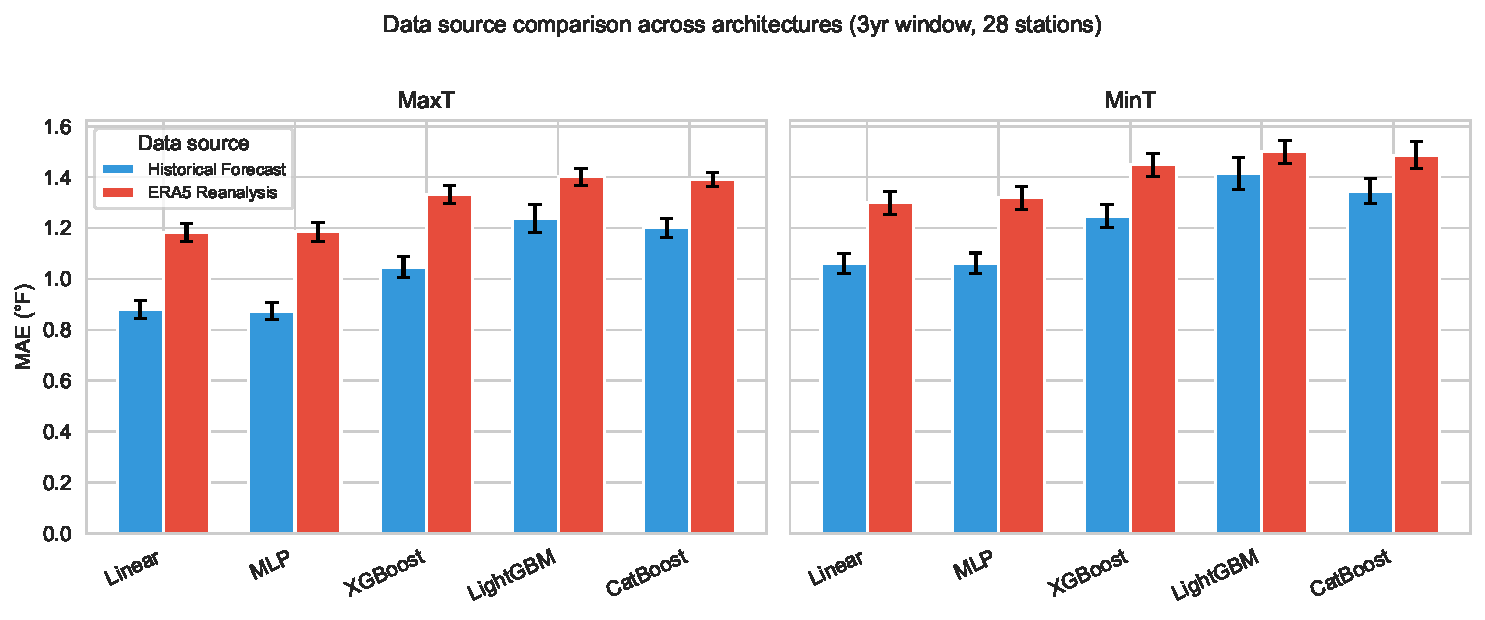
\includegraphics[width=33pc]{fig1_data_source_comparison.pdf}\\
  \caption{Data source comparison: Historical Forecast vs.\ ERA5 Reanalysis
  across all five architectures (3-year window, 28~stations). Error bars show
  $\pm 1$~SE. HF training data yields lower MAE for every architecture.}\label{fig:data_source}
\end{figure}

\subsection{Architecture Comparison (RQ3)}
\label{sec:results_arch}

Table~\ref{tab:architecture} presents mean MAE by architecture using historical
forecasts with a 3-year training window. The MLP achieves the lowest MaxT MAE
(0.874\textdegree{}F) and linear regression achieves the lowest MinT MAE
(1.061\textdegree{}F). Critically, the difference between MLP and linear is not
statistically significant ($p = 0.21$ for MaxT, $p = 0.42$ for MinT), while both
significantly outperform all three tree-based models ($p < 0.001$ in all cases).

\begin{table}[t]
\caption{Architecture comparison: mean MAE (\textdegree{}F) $\pm$ SE across
28~stations (historical forecast, 3-year window). Pairwise Wilcoxon $p$-values
are against the best architecture (boldface).}\label{tab:architecture}
\begin{center}
\begin{tabular}{lcccc}
\topline
Architecture & MaxT MAE & $p$ vs best & MinT MAE & $p$ vs best \\
\midline
\textbf{MLP}      & \textbf{0.874 $\pm$ 0.034} & ref    & 1.062 $\pm$ 0.040 & 0.42 \\
\textbf{Linear}   & 0.879 $\pm$ 0.036          & 0.21   & \textbf{1.061 $\pm$ 0.041} & ref \\
XGBoost            & 1.046 $\pm$ 0.041          & $<$0.001 & 1.247 $\pm$ 0.047 & $<$0.001 \\
CatBoost           & 1.200 $\pm$ 0.039          & $<$0.001 & 1.345 $\pm$ 0.049 & $<$0.001 \\
LightGBM           & 1.238 $\pm$ 0.055          & $<$0.001 & 1.415 $\pm$ 0.063 & $<$0.001 \\
\botline
\end{tabular}
\end{center}
\end{table}

\begin{figure}[t]
  \noindent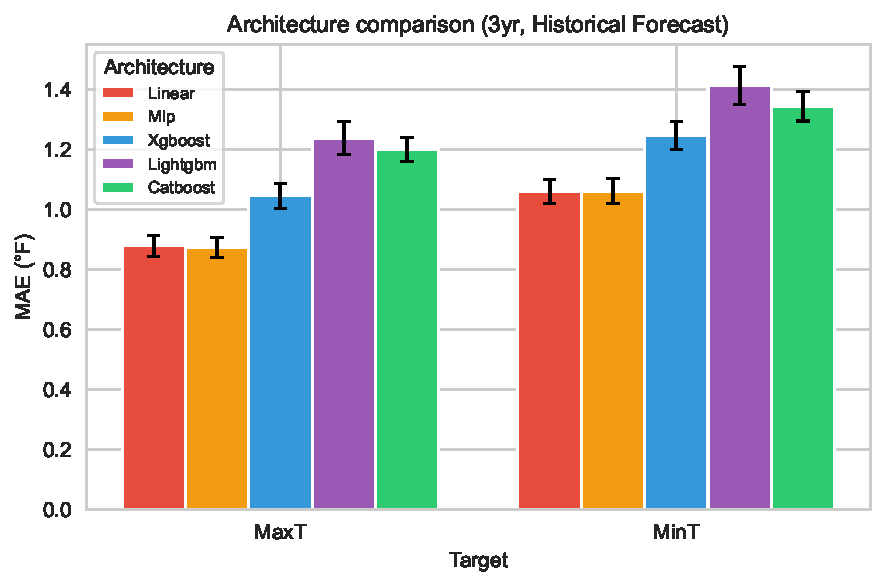
\includegraphics[width=27pc]{fig2_architecture_comparison.pdf}\\
  \caption{Architecture comparison (3-year, Historical Forecast). Error bars
  show $\pm 1$~SE across 28~stations.}\label{fig:architecture}
\end{figure}

\subsection{Training Window Sensitivity (RQ4)}
\label{sec:results_window}

Figures~\ref{fig:window_maxt} and~\ref{fig:window_mint} show MAE as a function of
training window length for each architecture. Two distinct patterns emerge:

\begin{itemize}
  \item \textbf{Linear and MLP}: MAE is relatively stable from 2--8 years, with
    near-optimal performance at 3~years (MaxT: 0.88\textdegree{}F; MinT:
    1.06\textdegree{}F). Additional data beyond 3~years provides negligible benefit.
  \item \textbf{Tree-based models}: MAE decreases substantially from 1~year
    (1.61--1.66\textdegree{}F for MaxT) to 5~years (1.04--1.06\textdegree{}F),
    reflecting the higher data requirements of nonparametric methods. Performance
    plateaus or slightly degrades at 8~years, possibly due to NWP model version
    changes in older data.
\end{itemize}

\begin{figure}[t]
  \noindent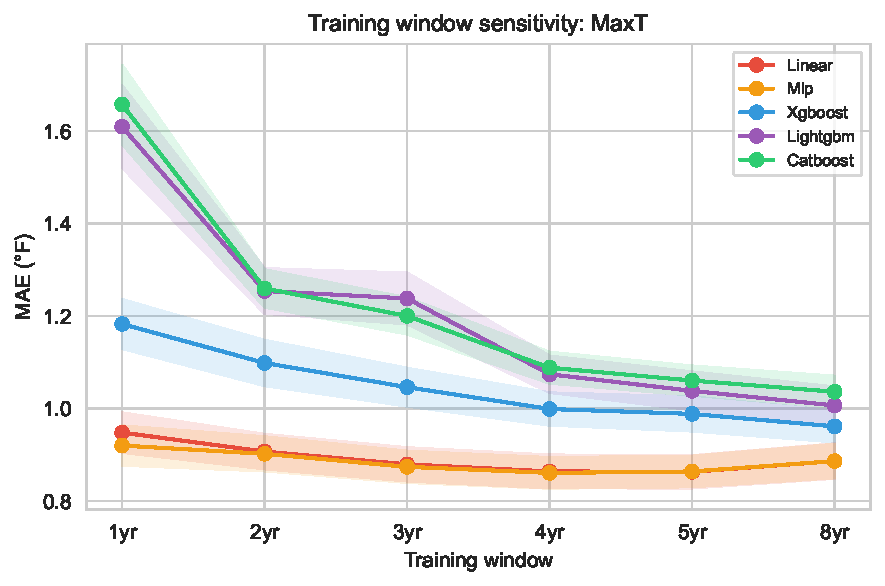
\includegraphics[width=27pc]{fig3_window_sensitivity_maxt.pdf}\\
  \caption{Training window sensitivity: MaxT. Shaded bands show $\pm 1$~SE
  across 28~stations.}\label{fig:window_maxt}
\end{figure}

\begin{figure}[t]
  \noindent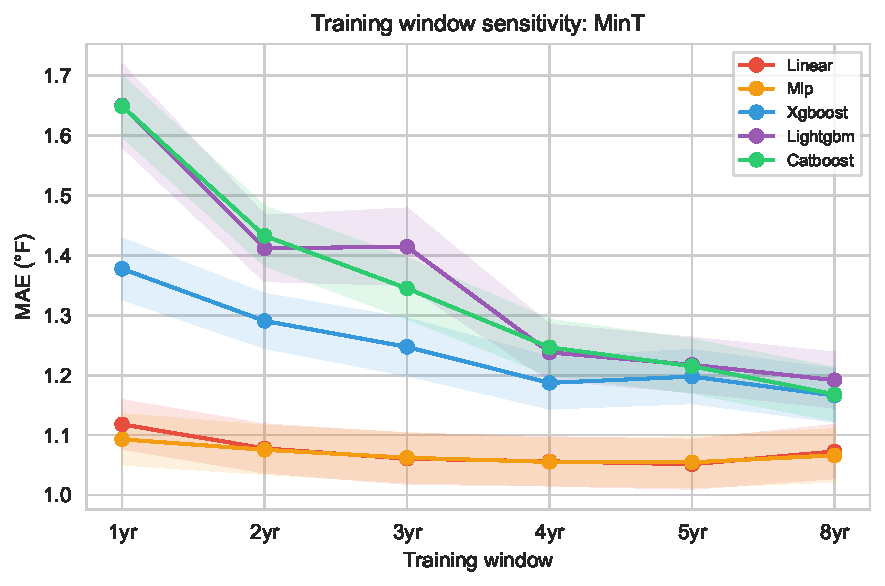
\includegraphics[width=27pc]{fig4_window_sensitivity_mint.pdf}\\
  \caption{Training window sensitivity: MinT.}\label{fig:window_mint}
\end{figure}

\subsection{MOS Skill vs.\ Raw NWP}
\label{sec:results_baseline}

Table~\ref{tab:baseline} compares the best ML post-processing model against raw
NWP baselines averaged over 28~stations. The best MOS model achieves an MAE of
0.87\textdegree{}F for MaxT and 1.05\textdegree{}F for MinT, representing a
\textbf{35\% improvement over raw GFS} (the primary freely available NWP baseline)
and 52\% over the GFS--ECMWF blend ($p < 0.001$ for all comparisons). ECMWF raw
MAE is also shown for completeness, though we note that ECMWF availability through
the Open-Meteo API is less consistent than GFS (see section~\ref{sec:limitations}),
and the GFS comparison should be treated as the primary benchmark.

\begin{table}[t]
\caption{Mean MAE (\textdegree{}F) across 28~stations: raw NWP vs.\ best MOS model.}\label{tab:baseline}
\begin{center}
\begin{tabular}{lcccc}
\topline
Target & GFS & ECMWF & Blend & Best MOS \\
\midline
MaxT & 1.335 & 2.601 & 1.826 & \textbf{0.868} \\
MinT & 1.664 & 2.212 & 1.769 & \textbf{1.053} \\
\botline
\end{tabular}
\end{center}
\end{table}

Table~\ref{tab:baseline_climate} breaks down the improvement by climate type.
Skill scores (defined as $\text{SS} = 1 - \text{MAE}_\text{model} /
\text{MAE}_\text{GFS}$) range from 0.11 (Continental MaxT) to 0.55 (SE
Subtropical MaxT), with higher skill generally in climates where GFS raw
errors are largest.

\begin{table}[t]
\caption{MOS skill vs.\ raw GFS by climate type: mean MAE (\textdegree{}F)
and skill score (SS = $1 - \text{model}/\text{GFS}$).}\label{tab:baseline_climate}
\begin{center}
\begin{tabular}{lcccccc}
\topline
 & \multicolumn{3}{c}{MaxT} & \multicolumn{3}{c}{MinT} \\
Climate & GFS & Model & SS & GFS & Model & SS \\
\midline
Continental      & 1.04 & 0.90 & 0.11 & 1.60 & 1.15 & 0.25 \\
NE Coastal       & 1.15 & 0.91 & 0.19 & 2.12 & 1.16 & 0.43 \\
SE Subtropical   & 2.00 & 0.86 & 0.55 & 1.47 & 0.98 & 0.28 \\
Gulf/SC          & 1.20 & 0.81 & 0.27 & 1.62 & 1.10 & 0.22 \\
Pacific          & 1.39 & 1.00 & 0.27 & 1.73 & 0.93 & 0.42 \\
Arid             & 1.01 & 0.65 & 0.24 & 1.33 & 0.78 & 0.41 \\
\botline
\end{tabular}
\end{center}
\end{table}

\begin{figure}[t]
  \noindent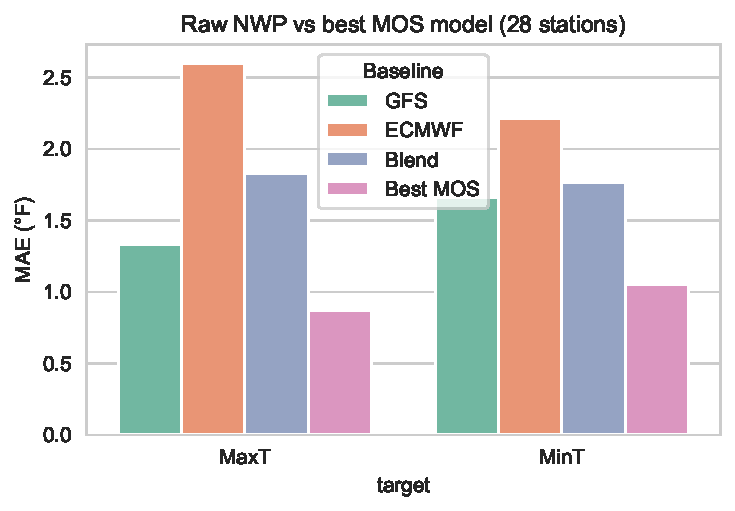
\includegraphics[width=19pc]{fig5_baseline_comparison.pdf}
  \noindent\includegraphics[width=19pc]{fig5b_skill_score_by_climate.pdf}\\
  \caption{(left) Mean MAE: raw NWP baselines vs.\ best MOS model (28~stations).
  (right) MOS skill score relative to raw GFS by climate type.}\label{fig:baseline}
\end{figure}

The SE~Subtropical region shows the highest MaxT skill (0.55), consistent with
the large raw GFS errors in that region (2.00\textdegree{}F). NE~Coastal stations
show the highest MinT skill (0.43), driven by large wintertime GFS MinT errors
(2.12\textdegree{}F). The per-station breakdown is provided in the supplementary
materials.

\subsection{Feature Importance and Ablation}
\label{sec:results_features}

\paragraph{Feature importance.}
Table~\ref{tab:features} reports the top features by model-averaged importance for
MaxT and MinT. NWP primary predictors dominate: \texttt{GFS\_MaxT} (36.8\%) and
\texttt{Forecast\_MaxT} (17.3\%) together account for over half of the total
importance for MaxT, with a similar pattern for MinT.

\begin{table}[t]
\caption{Top 10 features by mean importance (\%) across architectures.}\label{tab:features}
\begin{center}
\begin{tabular}{clr@{\hspace{2em}}clr}
\topline
\multicolumn{3}{c}{MaxT} & \multicolumn{3}{c}{MinT} \\
\# & Feature & Imp.\% & \# & Feature & Imp.\% \\
\midline
1 & GFS\_MaxT        & 36.8 & 1 & GFS\_MinT        & 31.6 \\
2 & Forecast\_MaxT   & 17.3 & 2 & Forecast\_MinT   & 16.2 \\
3 & EC\_MaxT         &  3.9 & 3 & GFS\_MeanT       &  5.9 \\
4 & GFS\_MeanT       &  2.8 & 4 & EC\_MinT         &  5.3 \\
5 & Bias\_MaxT\_Roll &  2.3 & 5 & Forecast\_MeanT  &  2.8 \\
6 & Forecast\_MeanT  &  1.9 & 6 & EC\_MeanT        &  2.1 \\
7 & Bias\_MaxT       &  1.7 & 7 & Bias\_MinT       &  2.0 \\
8 & EC\_MeanT        &  1.7 & 8 & Forecast\_DewPt  &  1.9 \\
9 & Uncertainty      &  1.4 & 9 & Bias\_MinT\_Roll &  1.6 \\
10 & Bias\_MinT\_Roll &  1.3 & 10 & MinT\_Roll7d    &  1.3 \\
\botline
\end{tabular}
\end{center}
\end{table}

\begin{figure}[t]
  \noindent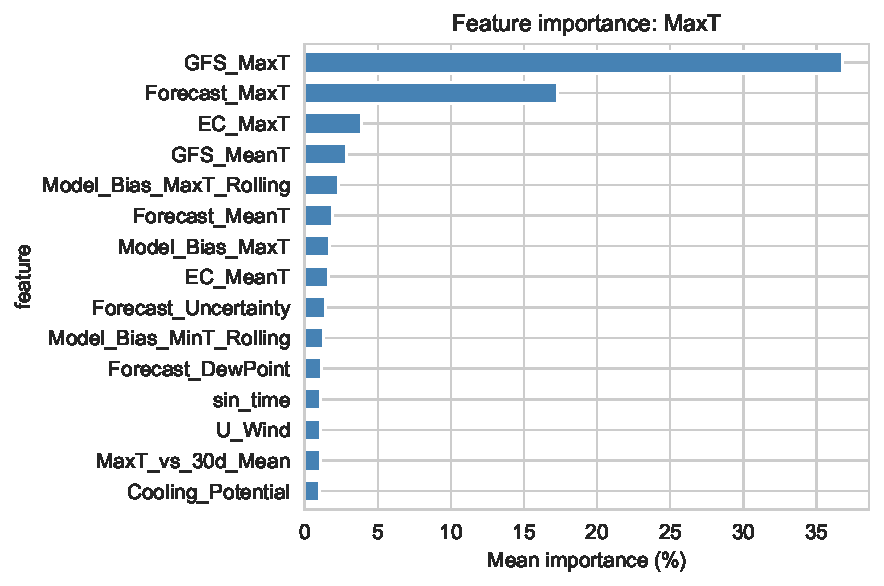
\includegraphics[width=19pc]{fig6_feature_importance_maxt.pdf}
  \noindent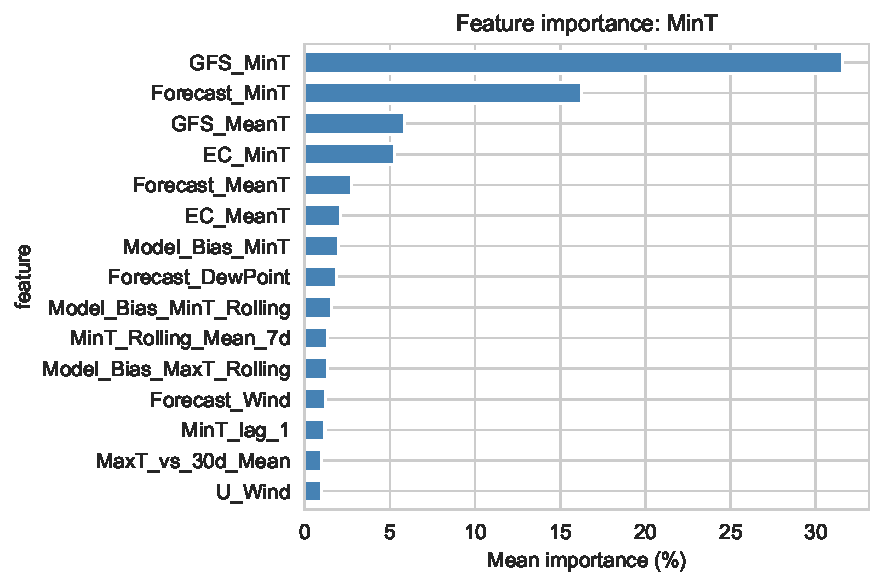
\includegraphics[width=19pc]{fig7_feature_importance_mint.pdf}\\
  \caption{Top 15 features by mean importance across architectures.
  (left) MaxT feature importance. (right) MinT feature importance.}\label{fig:feature_importance}
\end{figure}

\paragraph{Feature ablation.}
Figure~\ref{fig:ablation} presents the mean change in MAE ($\Delta$MAE) when each
feature group is removed, computed across 28~stations (Wilcoxon significance markers
shown). Positive values indicate degradation (the group was helpful). Key findings:

\begin{itemize}
  \item \textbf{NWP Primary}: Removing the core NWP temperature predictors causes
    the largest degradation across all architectures: 0.36--0.47\textdegree{}F for
    MaxT trees, 0.38--0.49\textdegree{}F for MinT ($p < 0.001$ in all cases).
    This sanity check confirms that NWP guidance is the essential input.
  \item \textbf{Bias Correction}: The only supplementary group that
    \emph{consistently} improves performance when present. Removing it degrades
    Linear and MLP by 0.037--0.041\textdegree{}F for MaxT ($p < 0.001$) and
    0.038--0.039\textdegree{}F for MinT ($p < 0.001$). Tree models show smaller,
    often non-significant effects.
  \item \textbf{Rolling Statistics and Lags}: Removing these groups often
    \emph{improves} tree model MAE (negative $\Delta$MAE), suggesting that
    tree models overfit to these features. Linear and MLP show near-zero effects.
  \item \textbf{ECMWF, Time, Physics}: Small and generally non-significant effects
    across all architectures.
\end{itemize}

\begin{figure}[t]
  \noindent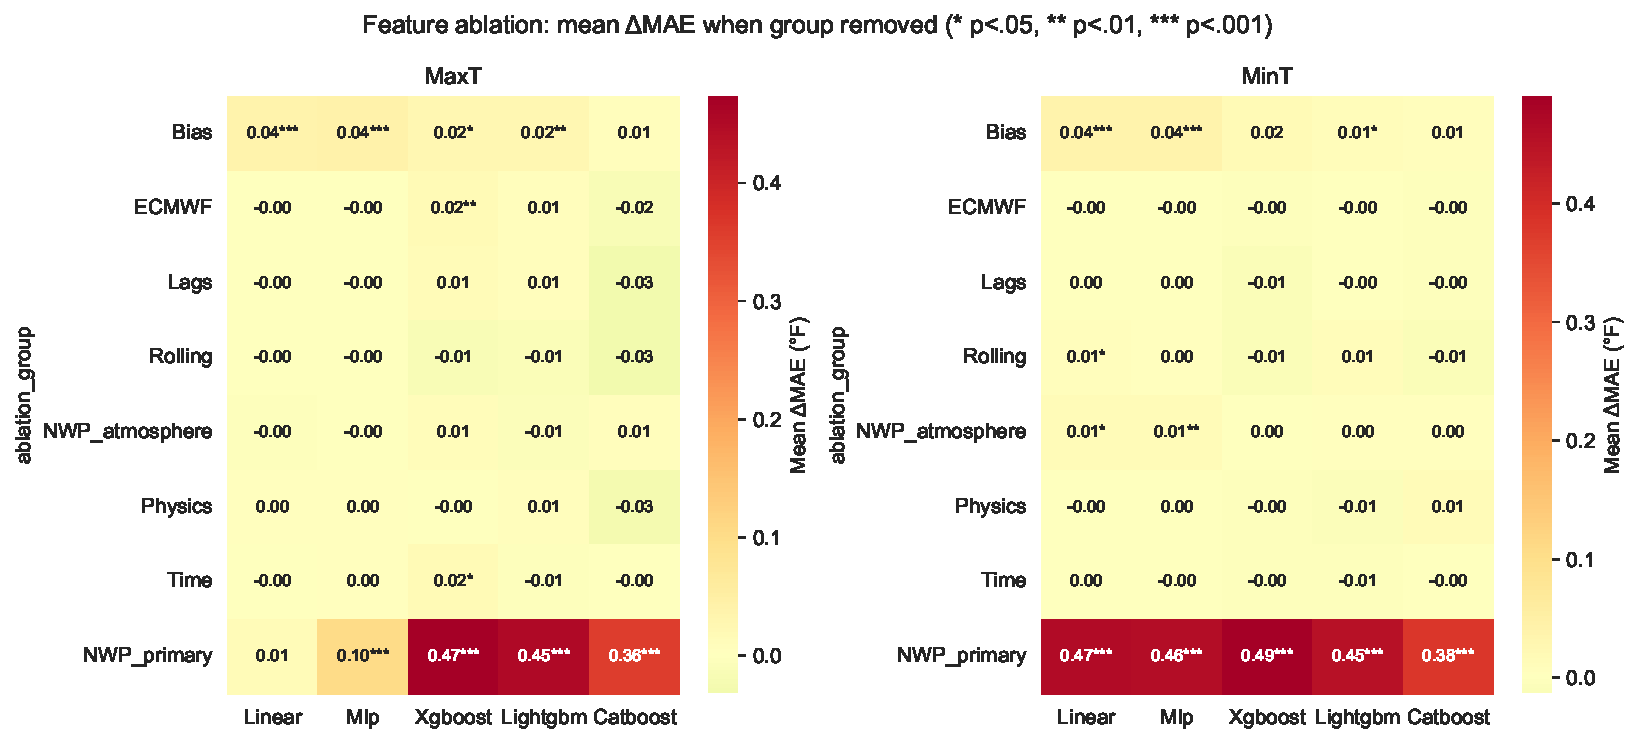
\includegraphics[width=33pc]{fig9_ablation_delta_mae.pdf}\\
  \caption{Feature ablation: mean $\Delta$MAE (\textdegree{}F) when each feature
  group is removed. Positive = worse without the group. Significance markers:
  $^{*}p < 0.05$, $^{**}p < 0.01$, $^{***}p < 0.001$ (Wilcoxon test across
  28~stations).}\label{fig:ablation}
\end{figure}

\subsection{Seasonal Analysis}
\label{sec:results_seasonal}

Table~\ref{tab:seasonal} and Fig.~\ref{fig:seasonal} present MAE by season for
the linear model (3-year historical forecast). MaxT performance is best in fall
(0.82\textdegree{}F) and worst in winter (0.95\textdegree{}F). MinT shows a
stronger seasonal signal, with summer performance (0.90\textdegree{}F)
substantially better than winter (1.30\textdegree{}F), likely reflecting larger
NWP errors during cold-season inversions and radiative cooling events.

\begin{table}[t]
\caption{Seasonal MAE (\textdegree{}F) for the linear model (3-year HF,
28~stations). SE computed across station-days.}\label{tab:seasonal}
\begin{center}
\begin{tabular}{lcccccc}
\topline
 & \multicolumn{3}{c}{MaxT} & \multicolumn{3}{c}{MinT} \\
Season & MAE & SE & $n$ & MAE & SE & $n$ \\
\midline
Summer (Jul--Sep) & 0.911 & 0.015 & 2564 & 0.897 & 0.015 & 2564 \\
Fall (Oct--Dec)   & 0.816 & 0.013 & 2576 & 1.113 & 0.020 & 2576 \\
Winter (Jan--Feb) & 0.945 & 0.038 & 1173 & 1.299 & 0.033 & 1173 \\
\botline
\end{tabular}
\end{center}
\end{table}

\begin{figure}[t]
  \noindent\includegraphics[width=19pc]{fig10_seasonal_mae.pdf}
  \noindent\includegraphics[width=19pc]{fig10b_monthly_mae.pdf}\\
  \caption{Seasonal and monthly MAE breakdown (Linear, 3-year HF, 28~stations).
  (left) Seasonal MAE. (right) Monthly MAE.
  Error bars / shaded bands show $\pm 1$~SE.}\label{fig:seasonal}
\end{figure}

We note that the test period (July 2025--February 2026) does not include spring
(March--June), and these results should be interpreted accordingly.

% ======================================================================
\section{Discussion}
\label{sec:discussion}

\subsection{Why Historical Forecasts Outperform Reanalysis}

The consistent MAE improvement from using historical forecasts as training data---
observed for every architecture and target combination tested ($p < 0.001$ in all
cases)---is both statistically significant and practically meaningful. The underlying
mechanism is straightforward: historical forecasts contain the same systematic
biases present in the operational NWP output the model seeks to correct. ERA5
reanalysis, by contrast, represents the best estimate of what actually occurred
and does not contain these forecast-specific error patterns. Training on historical
forecasts allows the ML model to learn a direct mapping from biased forecast to
observed truth, effectively learning the forecast model's error structure.

Crucially, this effect is not artefact of any particular model family: the
improvement is statistically significant for simple linear models, MLPs, and all
three gradient-boosted tree implementations alike. This universality strongly
suggests that the benefit derives from the training \emph{signal}, not from
interactions between the data source and a specific model's inductive bias.

This finding aligns with the classical MOS philosophy \citep{glahn1972mos} and
suggests that the modern trend toward reanalysis-based training represents a
methodological regression, not an advance.

\subsection{Why Simple Models Suffice}

The finding that linear regression and a small MLP match or outperform
gradient-boosted trees is perhaps surprising given the dominance of tree-based
methods in many ML benchmarks. We offer two explanations:

First, temperature post-processing operates in a \emph{low-noise regime}: the
NWP forecast is already a strong predictor (explaining $>$90\% of variance), and
the residual correction is primarily a bias adjustment. In such settings, simple
models with strong inductive bias toward linear relationships are well-suited,
while complex models risk overfitting to noise.

Second, the ablation results support this interpretation. Tree models show negative
$\Delta$MAE when rolling statistics and lagged observations are removed, meaning
these features actively harm performance. Tree models, with their capacity to
memorize complex interactions, apparently learn spurious patterns from these noisy
features. Linear models, constrained to additive effects, are immune to this
failure mode.

\subsection{Practical Guidance}

Based on these results, we offer the following recommendations for practitioners:

\begin{enumerate}
  \item \textbf{Use historical forecasts, not reanalysis}, as training data for ML
    post-processing. The Open-Meteo Historical Forecast API provides free access to
    multi-year GFS and ECMWF forecast archives.
  \item \textbf{Start with linear regression} or a small MLP. These match the
    performance of more complex models while being faster to train, easier to
    interpret, and less prone to overfitting.
  \item \textbf{Three years of recent data} is sufficient for near-optimal
    performance with linear models. Gradient-boosted trees benefit from longer
    windows (5+ years) but still underperform simple models.
  \item \textbf{Include bias-correction features} (yesterday's forecast error and
    its rolling mean) as predictors. These are the only supplementary features that
    consistently improve performance across all architectures.
\end{enumerate}

\subsection{Limitations}
\label{sec:limitations}

Several limitations should be noted:

\begin{itemize}
  \item \textbf{Single test period}: All experiments share the same 227-day test
    period (July 2025--February 2026), which excludes spring and early summer
    (March--June). This design reflects the operational context of the study: the
    Kalshi temperature prediction markets are a recent development, and the test
    period represents a real-time forward evaluation of the system as it would
    operate in production. Multi-year cross-validation would require historical
    forecast data extending back to at least 2019 (to allow 3-year training windows
    with separate test years), but the Open-Meteo Historical Forecast API provides
    reliable GFS archives only from approximately 2022 onward for most stations.
    Future work should extend the evaluation as more years of historical forecast
    data become available.
  \item \textbf{Temperature only}: We evaluate MaxT and MinT. Temperature
    post-processing is relatively linear, and the finding that simple models suffice
    may not generalize to discontinuous or highly skewed variables such as
    precipitation or wind gusts, which may benefit from the flexibility of
    tree-based or deep learning approaches.
  \item \textbf{U.S.\ stations only}: All 28~stations are in the contiguous United
    States, selected for their correspondence to active Kalshi markets. Results may
    differ for tropical, polar, or maritime climates not represented here.
  \item \textbf{ECMWF data quality}: The raw ECMWF MAE (2.60\textdegree{}F for
    MaxT) is higher than expected and likely reflects incomplete ECMWF IFS
    availability through the Open-Meteo API rather than true ECMWF forecast skill.
    The ECMWF model transitioned from IFS to IFS-0.25\textdegree{} in 2024, and
    coverage gaps in the API archive may disproportionately affect our test period.
    For this reason, we treat \textbf{raw GFS as the primary NWP baseline}
    throughout this study.
  \item \textbf{Deterministic focus}: We use quantile regression for uncertainty
    quantification but do not evaluate full probabilistic skill (e.g., CRPS).
\end{itemize}

% ======================================================================
\section{Conclusions}
\label{sec:conclusions}

This study provides the first systematic comparison of historical forecasts vs.\
ERA5 reanalysis as training data for ML-based Model Output Statistics, evaluated
across 28~U.S.\ stations, five ML architectures, six training windows, and
eight feature ablation conditions. Three principal findings emerge:

\begin{enumerate}
  \item \textbf{Training data source matters more than model architecture.}
    Historical forecasts reduce MAE by 6--26\% compared to ERA5 reanalysis
    ($p < 0.01$ in 9 of 10 architecture--target combinations), with the
    largest gains for simple models (MLP: 26\%, Linear: 26\% on MaxT). This
    result is consistent across all six climate types and demonstrates that the
    benefit stems from the training signal, not model-specific interactions.
  \item \textbf{Simple models are sufficient for temperature post-processing.}
    Linear regression and a small MLP achieve the lowest MAE (0.87--0.88\textdegree{}F
    for MaxT, 1.06\textdegree{}F for MinT) and are not significantly different from
    each other. Both significantly outperform XGBoost, LightGBM, and CatBoost.
  \item \textbf{Three years of recent forecast data is near-optimal.}
    Linear/MLP performance plateaus at 3~years; longer windows provide no
    additional benefit. Tree models improve with more data but still underperform
    simple models even with 8~years of training data.
\end{enumerate}

The best ML post-processing model reduces MAE by 35\% over raw GFS and 52\% over
the GFS--ECMWF blend, with skill scores varying by climate type from 0.11
(Continental MaxT) to 0.55 (SE Subtropical MaxT). Feature ablation confirms that
NWP primary predictors and bias-correction features are essential, while rolling
statistics and lagged observations can harm tree-based models through overfitting.

These results provide actionable guidance for the operational weather forecasting
community and for participants in weather prediction markets: use freely available
historical forecast APIs rather than reanalysis, prefer simple models, and invest
in bias-correction features rather than complex architectures.

Future work should extend this analysis to additional forecast variables (wind,
dew point, precipitation), international station networks, and ensemble-based
post-processing methods.

\clearpage
%%%%%%%%%%%%%%%%%%%%%%%%%%%%%%%%%%%%%%%%%%%%%%%%%%%%%%%%%%%%%%%%%%%%%
% ACKNOWLEDGMENTS
%%%%%%%%%%%%%%%%%%%%%%%%%%%%%%%%%%%%%%%%%%%%%%%%%%%%%%%%%%%%%%%%%%%%%
\acknowledgments
[To be completed.]

%%%%%%%%%%%%%%%%%%%%%%%%%%%%%%%%%%%%%%%%%%%%%%%%%%%%%%%%%%%%%%%%%%%%%
% DATA AVAILABILITY STATEMENT
%%%%%%%%%%%%%%%%%%%%%%%%%%%%%%%%%%%%%%%%%%%%%%%%%%%%%%%%%%%%%%%%%%%%%

\datastatement
Historical forecast and reanalysis data were obtained from the Open-Meteo API
(\url{https://open-meteo.com/}). Observations were obtained from the ACIS web
services (\url{https://www.rcc-acis.org/}). Code and experiment results are
available at [repository URL].

%%%%%%%%%%%%%%%%%%%%%%%%%%%%%%%%%%%%%%%%%%%%%%%%%%%%%%%%%%%%%%%%%%%%%
% APPENDIXES
%%%%%%%%%%%%%%%%%%%%%%%%%%%%%%%%%%%%%%%%%%%%%%%%%%%%%%%%%%%%%%%%%%%%%

\appendix

\appendixtitle{Supplementary Tables}

\subsection*{RMSE comparison}

\begin{table}[t]
\caption{Supplementary: mean RMSE (\textdegree{}F) by architecture and data source
(3-year training window, 28~stations). Layout mirrors Table~\ref{tab:data_source}.}\label{tab:supp_rmse}
\begin{center}
\begin{tabular}{llccc}
\topline
Target & Architecture & HF RMSE & ERA5 RMSE & Improv.\ (\%) \\
\midline
  \multirow{5}{*}{MaxT} & Linear & 1.170 & 1.548 & 24.4 \\
   & MLP & 1.165 & 1.554 & 25.0 \\
   & XGBoost & 1.487 & 1.800 & 17.4 \\
   & LightGBM & 2.078 & 2.003 & $-$3.7 \\
   & CatBoost & 1.713 & 1.868 & 8.3 \\
\midline
  \multirow{5}{*}{MinT} & Linear & 1.396 & 1.718 & 18.7 \\
   & MLP & 1.398 & 1.744 & 19.8 \\
   & XGBoost & 1.718 & 1.928 & 10.9 \\
   & LightGBM & 2.187 & 2.081 & $-$5.1 \\
   & CatBoost & 1.864 & 1.992 & 6.4 \\
\botline
\end{tabular}
\end{center}
\end{table}

%%%%%%%%%%%%%%%%%%%%%%%%%%%%%%%%%%%%%%%%%%%%%%%%%%%%%%%%%%%%%%%%%%%%%
% REFERENCES
%%%%%%%%%%%%%%%%%%%%%%%%%%%%%%%%%%%%%%%%%%%%%%%%%%%%%%%%%%%%%%%%%%%%%

\bibliographystyle{ametsocV6}
\bibliography{references}

\end{document}
